\section{La perception Kinesthésique}
\subsection{Perception}
\begin{frame}{La perception kinesthésique}

\begin{itemize}
\item Perception de la position des membres, du mouvement des muscles
\item par extension: force, poids, inertie
\end{itemize}

\begin{itemize}
\item Récepteurs kinesthésiques
\begin{itemize}
\item Fibres musculaires
\item Organes tendineux de Golgi
\item Mécanorecepteurs dans les articulations
\end{itemize}
\end{itemize}

\end{frame}

{
\setbeamertemplate{frame footer}{\copyright http://faculty.pasadena.edu}
\begin{frame}{La perception kinesthésique}
\begin{figure}
\centering
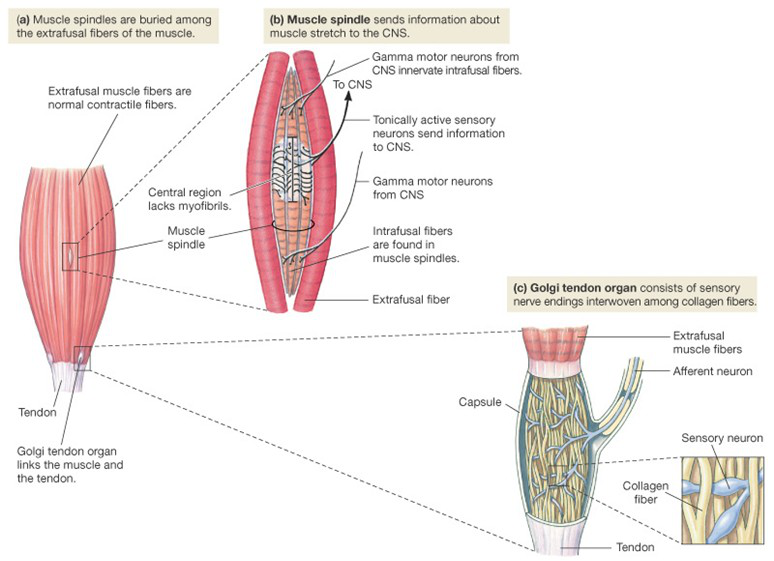
\includegraphics[width=10cm]{images/muscles}
\end{figure}
\end{frame}
}

{
\setbeamertemplate{frame footer}{\cite{Jones2000}}
\begin{frame}{La perception kinesthésique}
\begin{figure}
\centering
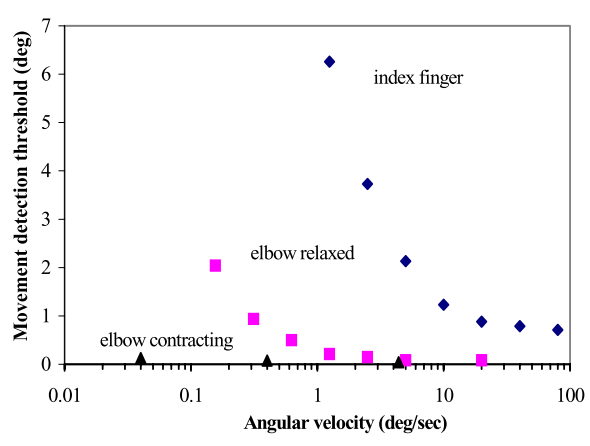
\includegraphics[width=9cm]{images/jnd_position}
\end{figure}
\end{frame}

\begin{frame}{La perception kinesthésique}
\begin{table}[]
\centering
\footnotesize
	\begin{tabular}[]{lcc}
		\toprule
		\textbf{Variable} & \textbf{Résolution} & \textbf{Seuil différentiel}\\
		\midrule
		Mouvement des membres & 0.5-1$^{\circ}$ & 8\% (intervalle 4-9\%)\\
		Position des membres & 0.8-7$^{\circ}$ & 7\% (intervalle 5-9\%)\\
		Force & 0.06N & 7\% (intervalle 5-12\%)\\
		Rigidité & - & 17\% (intervalle 8-22\%)\\
		Viscosité & - & 19\% (intervalle 14-34\%)\\
		Inertie & - & 28\% (intervalle 21-113\%)\\
		\bottomrule
	\end{tabular}
	\caption{Sensibilité kinesthésique}
\end{table}
\end{frame}
}

\subsection{Illusions kinesthésiques}
\begin{frame}{Illusions kinesthésiques}
\begin{multicols}{2}
\begin{itemize}
\item Pseudo-haptique
\begin{itemize}
\item illusion de retour de force
\item décalage entre mouvement et retour visuel attendu
\end{itemize}
\end{itemize}
\begin{figure}
\centering
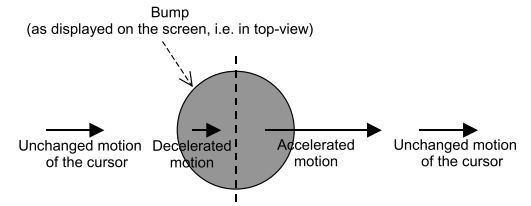
\includegraphics[width=5cm]{images/pseudoHaptic}
\caption{\cite{Lecuyer2009}}
\end{figure}
\end{multicols}
\begin{figure}
\centering
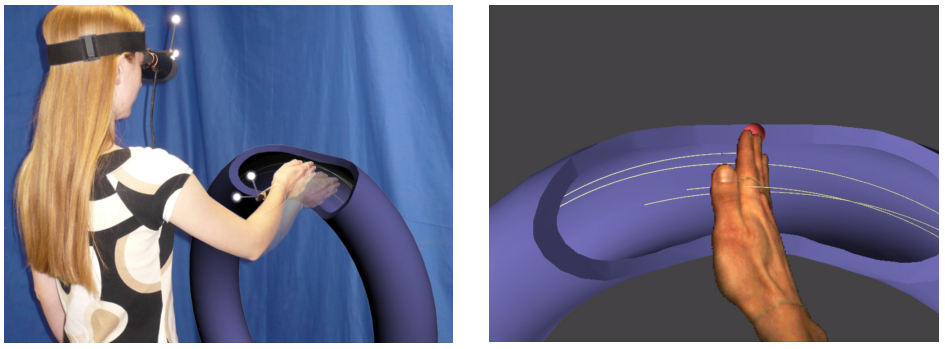
\includegraphics[width=9cm]{images/pseudoHaptic3D}
\caption{\cite{Pusch2008}}
\end{figure}
\end{frame}

{
\setbeamertemplate{frame footer}{\cite{Roll1995}}
\begin{frame}{Illusions kinesthésiques}
\begin{itemize}
\item Illusions de mouvement
\begin{itemize}
\item vibration sur tendon
\end{itemize}
\end{itemize}
\begin{figure}
\centering
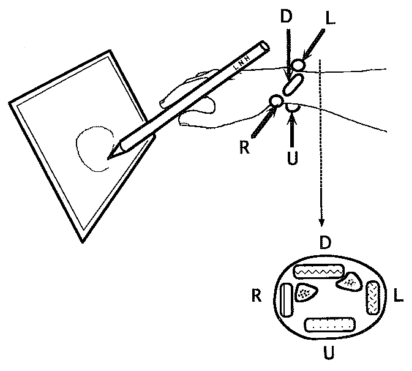
\includegraphics[width=5cm]{images/vibrationmovement}
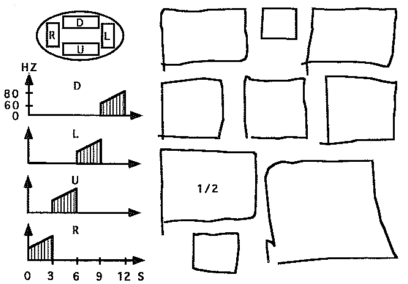
\includegraphics[width=5cm]{images/vibrationmovement2}
\end{figure}
\end{frame}
}

\subsection{Interface à retour de force}
\begin{frame}{Interface classique : bras à retour de force}
\begin{itemize}
\item Impédance (in: position, out: force)
\item Admittance (in: force, out: position)
\end{itemize}

\begin{multicols}{2}
\begin{figure}
\centering
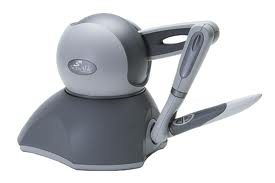
\includegraphics[width=4cm]{images/phantom}
\caption{\copyright 3dsystems.com}
\end{figure}
%
\begin{figure}
\centering
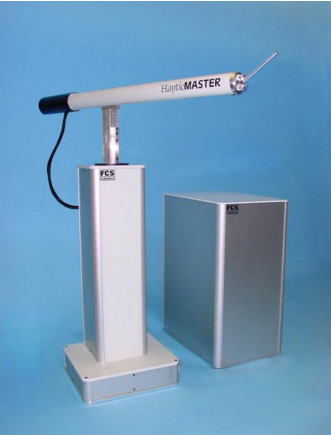
\includegraphics[width=4cm]{images/hapticMaster}
\caption{\cite{VanderLinde2002}}
\end{figure}
\end{multicols}
\end{frame}

\begin{frame}{Interfaces Avancées}
\begin{itemize}
\item Articulations complexes (ex: Sense glove, exosquelette)
\item Simulation électrique des muscles (ex: Impacto)
\item Espace de travail etendu (ex: SPIDAR)
\item Proxy / props (ex: haptic PIVOT \cite{kovacs2020haptic})
\item \url{https://haptipedia.org} \cite{seifi2019haptipedia}
\end{itemize}
\begin{multicols}{3}
\begin{figure}
\centering
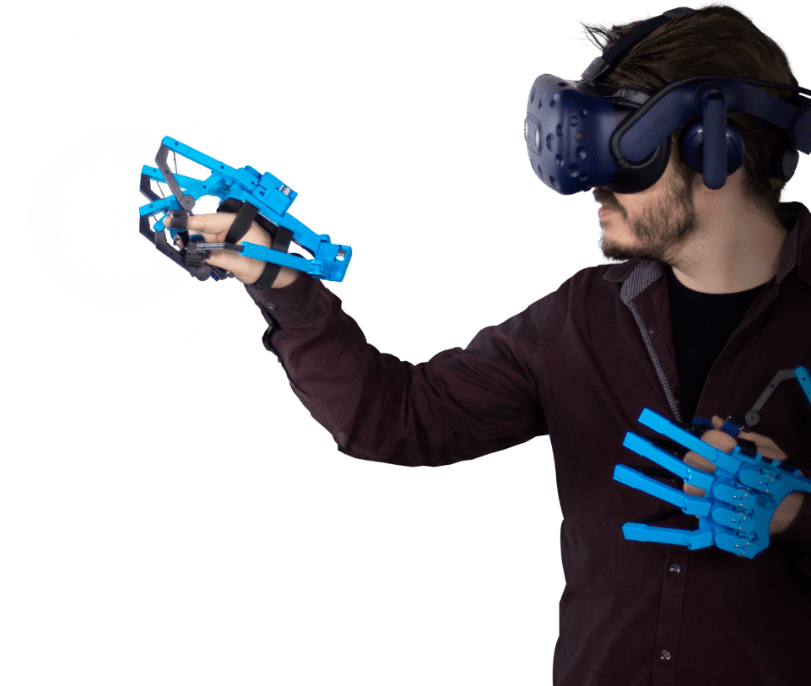
\includegraphics[width=3.7cm]{images/senseglove}
%\vspace{0.3cm}
\caption{\copyright senseglove.com}
\end{figure}
\begin{figure}
\centering
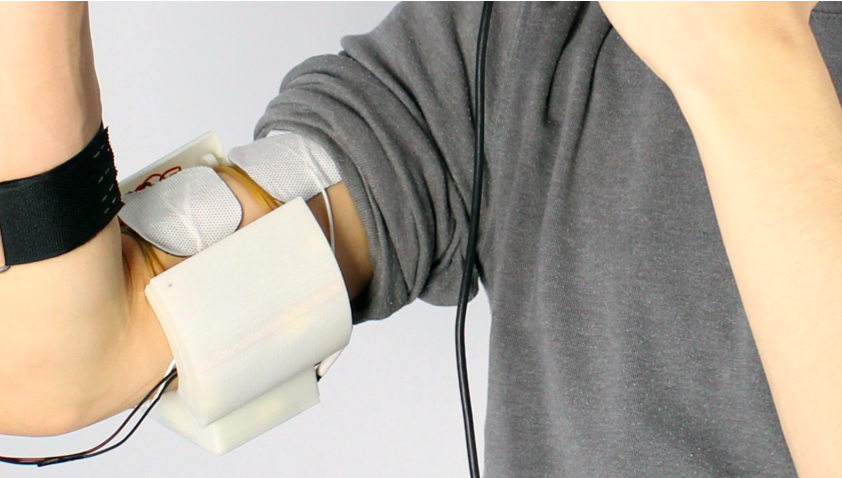
\includegraphics[width=3.7cm]{images/impacto}
%\vspace{0.85cm}
\caption{\cite{lopes2015}}
\end{figure}
\begin{figure}
\centering
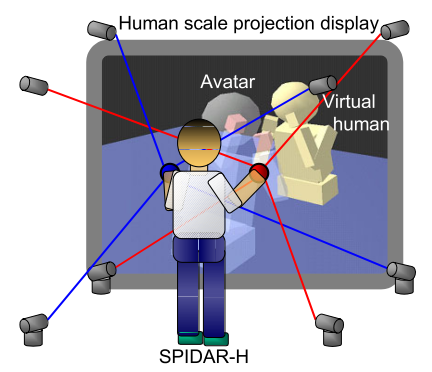
\includegraphics[width=3.5cm]{images/spidar}
\caption{\cite{Hasegawa2006a}}
\end{figure}
\end{multicols}
\end{frame}

{
\setbeamertemplate{frame footer}{\copyright \cite{kovacs2020haptic}}
\begin{frame}{Interfaces Avancées}
\begin{figure}
\href{run:videos/Haptic_PIVOT.mp4}{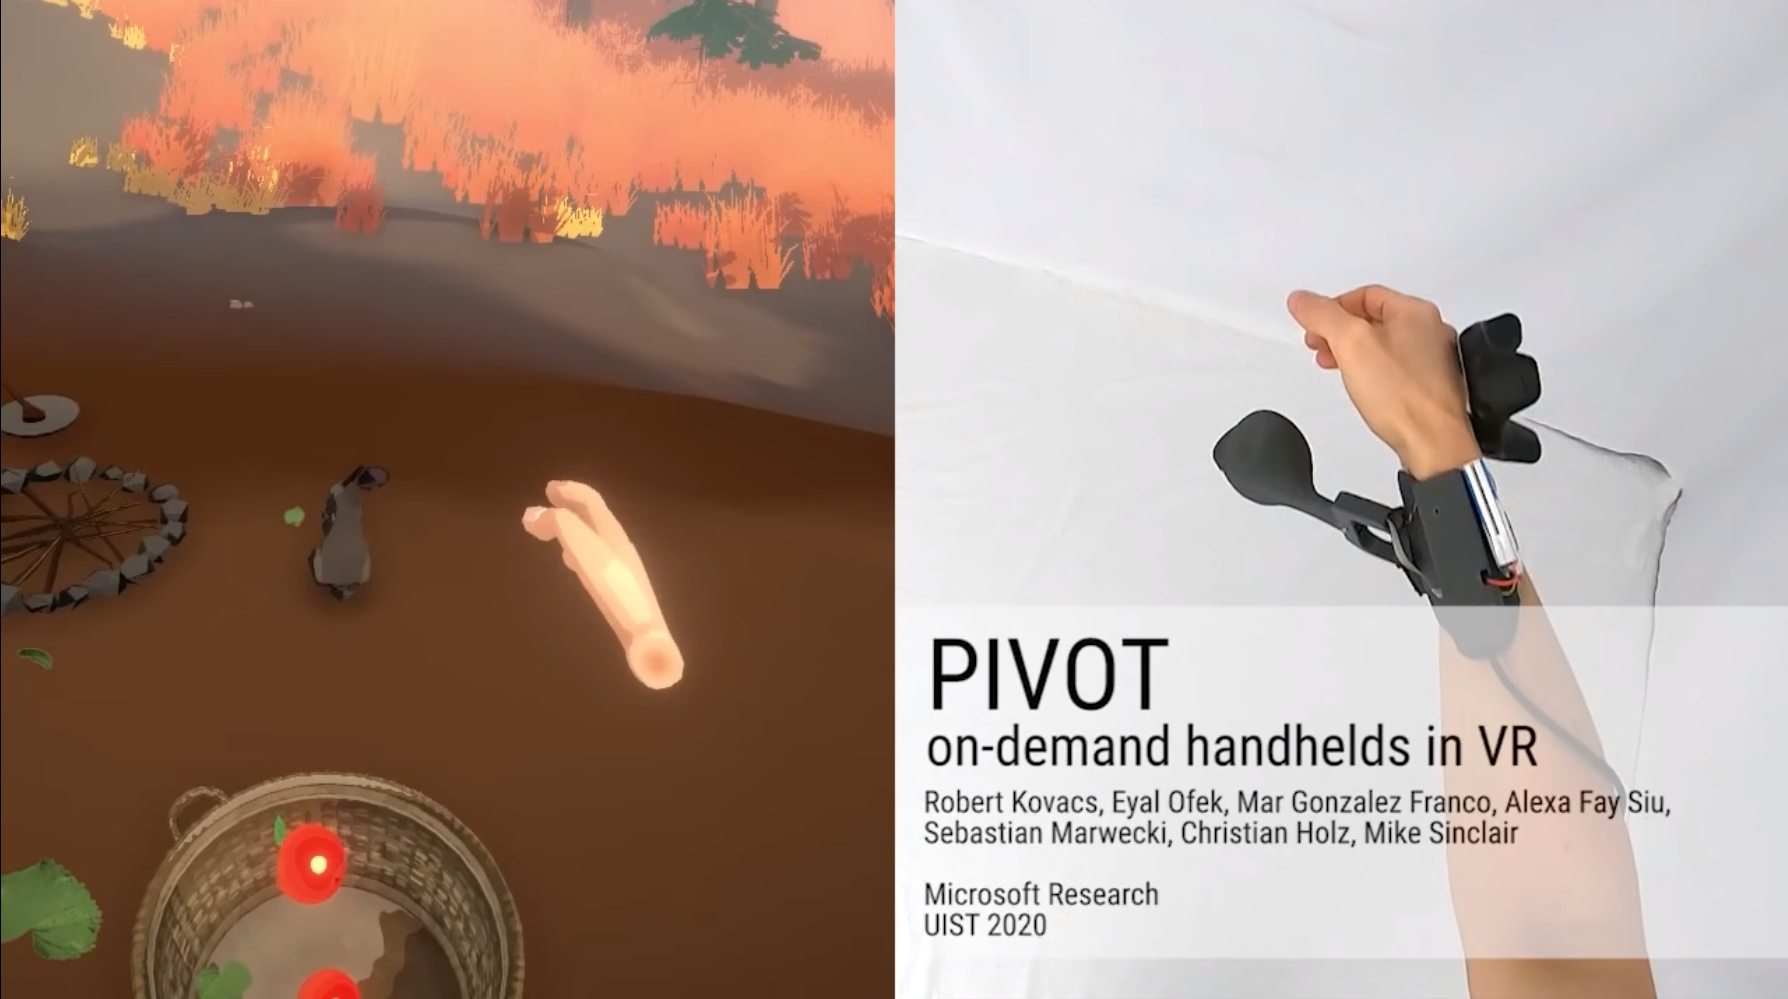
\includegraphics[width=\linewidth]{images/hapticPIVOT}}
\end{figure}
\end{frame}
}

\subsection{Rendu Haptique}
\begin{frame}{Rendu haptique}
\begin{itemize}
\item Calcul des forces résultant de l'interaction de l'utilisateur avec des objets virtuels
\end{itemize}
\begin{figure}
\centering
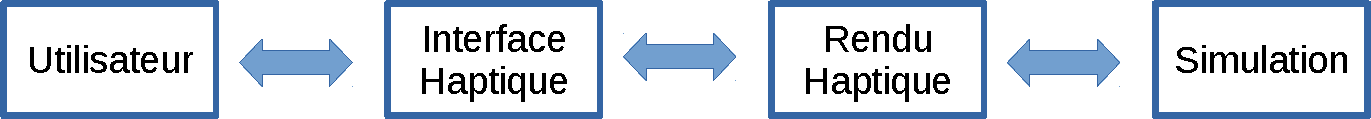
\includegraphics[width=\linewidth]{images/schema_haptique}	
\caption{Flux de travail pour l'interaction haptique}
		%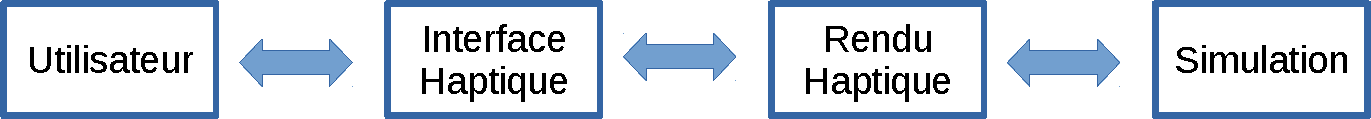
\includegraphics[width=4cm]{images/schema_haptique}{Johansson and Westling}
\end{figure}
\begin{itemize}
\item Algorithme de base (impédance)
\begin{itemize}
\item Acquisition de la position de l'interface haptique
\item Analyse d'éventuelles collisions avec des objets virtuels
\item Si collision, calculer les forces de réaction
\item Reproduire ces forces sur l'interface haptique et mise à jour de la simulation
\end{itemize}
\end{itemize}
\begin{itemize}
\item Fréquence de mise à jour idéale: $1kHz$
\end{itemize}
\end{frame}


\begin{frame}{Rendu haptique - Principe de base}
\begin{itemize}
\item Proxy contrôlé par bras à retour de force (impédance)
\item Exemple pour 1 degré de liberté
\end{itemize}
\begin{figure}
\centering
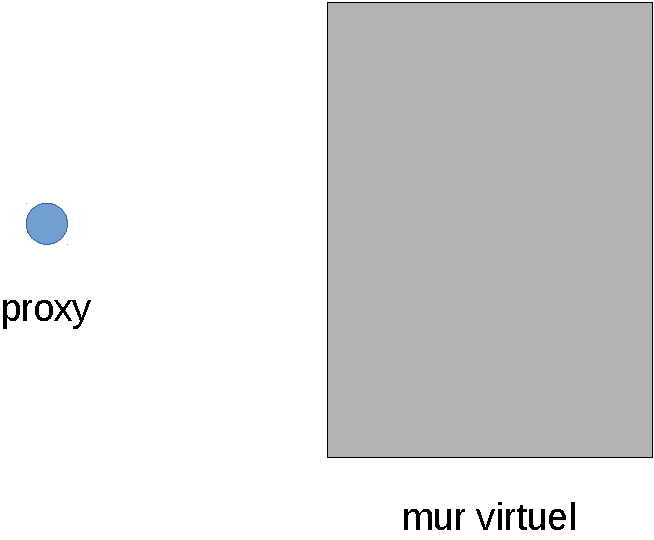
\includegraphics[width=7cm]{images/hapticRendering}{}
\end{figure}
\end{frame}

\begin{frame}{Rendu haptique - Principe de base}
\begin{itemize}
\item Collision modélisée par un ressort
\item $F = -Kd$, $K$ = rigidité du mur (stiffness)
\end{itemize}
\begin{figure}
\centering
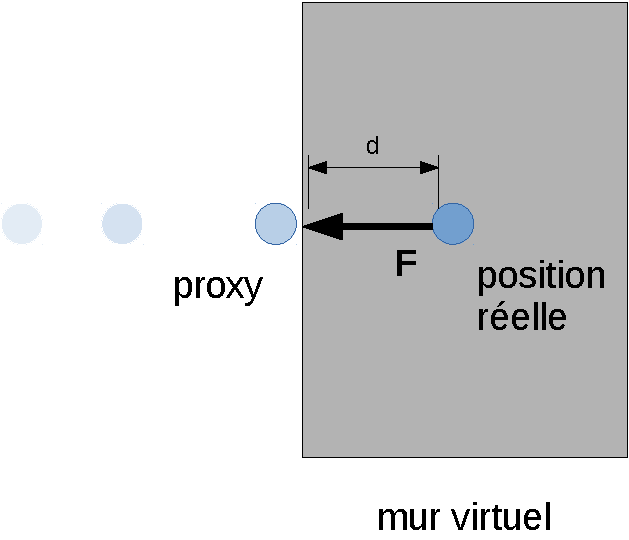
\includegraphics[width=7cm]{images/hapticRendering2}{}
\end{figure}
\end{frame}

\begin{frame}{Rendu haptique - Principe de base}
\begin{itemize}
\item Collision modélisée par un ressort et amortissement
\item $F = -Kd - Bv$, $K$ = stiffness, $B$ = amortissement (damping)
\end{itemize}
\begin{figure}
\centering
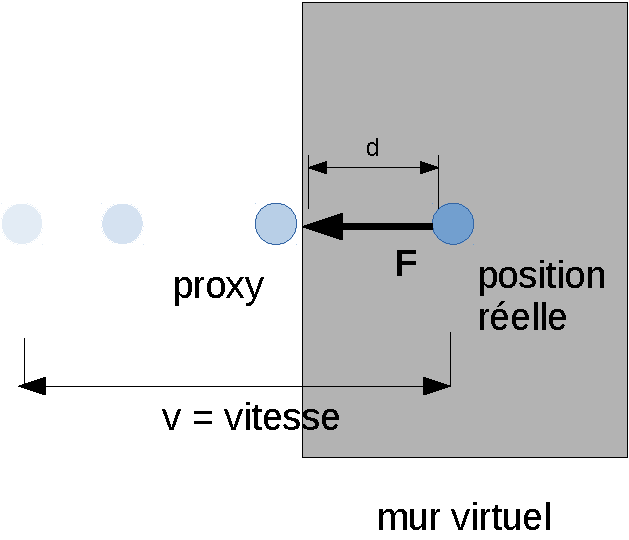
\includegraphics[width=7cm]{images/hapticRendering3}{}
\end{figure}
\end{frame}

\begin{frame}{Rendu haptique - Principe avancé}
\begin{itemize}
\item Objets virtuels complexes
\item 6 degrés de liberté
\end{itemize}
\begin{multicols}{2}
\begin{figure}
\centering
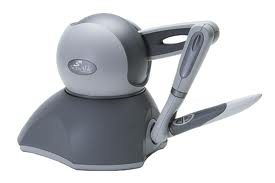
\includegraphics[width=5cm]{images/phantom}
\vspace{0.25cm}
\caption{\copyright geomagic.com}
\end{figure}
\begin{figure}
\centering
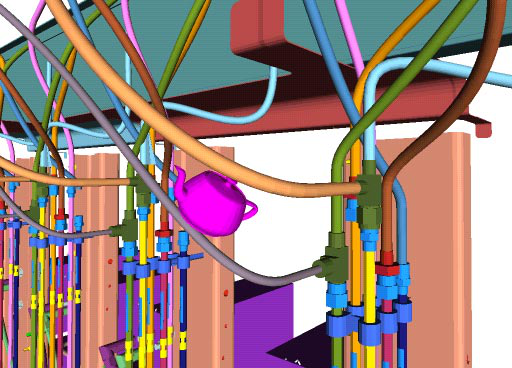
\includegraphics[width=5cm]{images/hapticRenderingExample}
\caption{\cite{McNeely2005}}
\end{figure}
\end{multicols}
\end{frame}

{
\setbeamertemplate{frame footer}{\cite{McNeely2006}}
\begin{frame}{Rendu haptique - Principe avancé}
\begin{itemize}
\item Découpage en "voxmap" et "pointshell"
\item Détection des collisions et calcul des forces locales
\item Calcul des forces liées au proxy
\end{itemize}
\begin{figure}
\centering
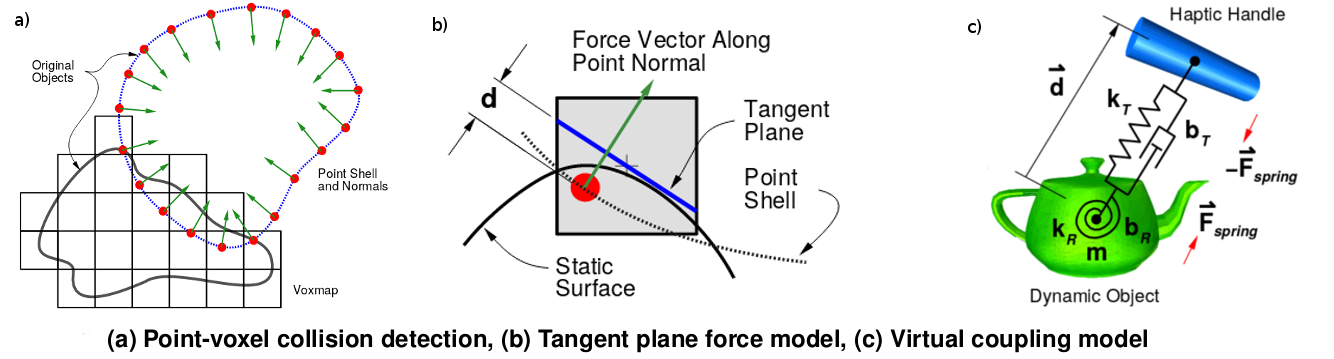
\includegraphics[width=\linewidth]{images/hapticVoxel_corrected}
\end{figure}
\end{frame}
}


%\subsection{Demo}
%{
%\setbeamertemplate{frame footer}{\copyright chai3d.org}
%\begin{frame}{Demo}
%\begin{itemize}
%\item Novint Falcon
%\item CHAI 3D API (C++)
%\begin{itemize}
%\item Interaction avec des corps solides
%\item Interaction avec des corps mous
%\end{itemize}
%\end{itemize}
%\begin{figure}
%\centering
%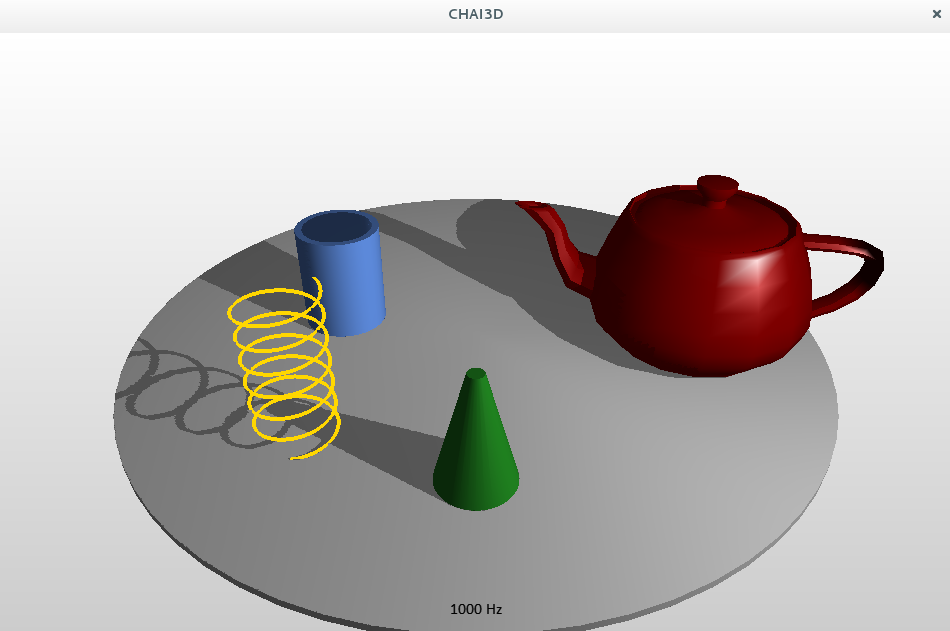
\includegraphics[width=5cm]{images/demo_solides}
%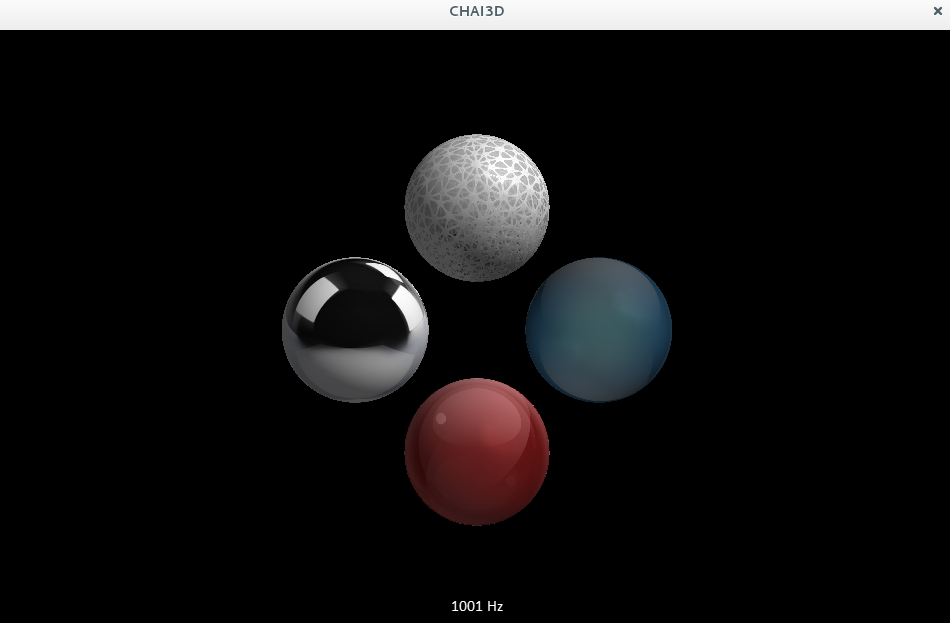
\includegraphics[width=5cm]{images/demo_textures}
%\end{figure}
%\end{frame}
%}